\chapter{Contraction Hierarchies}\label{chapter:ch}

Eine Methode um in Graphen, inbesondere in Straßengraphen, sehr schnell kürzeste Pfade zu berechen, sind Contraction Hierachies.
Die von \cite{geisberger2008contraction} vorgestellte Methode nutzt ein änliches Konzept zu dem in \autoref{graphs:strassengraphen} vorgestellten Level auf.
Die Grundidee der Suche eines kürzesten Pfades ist ein Bidirectionale Suche, welche jeweils nur höhere Level besucht.
Durch diese Enschränkung des Suchhraums kann, je nach dem Graphentyp, ein Speedup mehrerer größenordnungen erreicht werden.

Wie zu sehen sein wird, lassen sich die klassischen Methoden zur Erstellung der benötigten DAtenstrukturen nur bedingt auf Sichtbarkeitsgraphen anwenden.
Daher wird im follgenden zuerst unabhängig der Erstellung argumentiert.

Contraction Hierarchies bauen auf der Notation eines \emph{Levels} auf.
Jedem Knoten wird ein Level zugeorndet.
Diese kann als ein Grad der Wichtigkeit verstanden werden:
Je höher ein Level ist, desto wichtiger ist der Knoten im Allgemeinen für das finden von kürzesten Pfaden.

\begin{definition}[Level]
    Sei $G = V, E$ ein Graph.
    Sei $L \subseteq \mathbb{N}$ mit $\abs{L} = \abs{V}$.
    Dann wird eine bijketive Funktion ${vtl} \coloneq V \to L$ \emph{vertex-to-level} Funktion genannt.
    Ihre Umkehrfunktion ${ltv}$ wird \emph{level-to-vertex} Funktion genannt.
\end{definition}

Die ein Level aus genau einem Knoten besteht, ist keine zwingen Notwendigkeit
So setzt \cite{vetter2009parallel} etwa mehrere Knoten auf einem Level, um das Preprocessing zu beschleunigen.
Die in dieser Arbeit verwende Einschränkung vereinfacht allerdings die argumentation.

Bassierend auf dem Level kann der \emph{upward Graph} definiert werden.
Der Name des upward Graphen ergibt sich daher, dass die Suche in einem upward Graph auf das Level bezogen nur \emph{aufwärts} geht.
Formal ist dieser definiert als:

\begin{definition}[Upward Graph]
    Sei $G = (V, E)$ und ${vtl}$ eine \emph{vertex-to-level} Funktion dazu. Dann ist $G_u = (V, E_u)$ ein \emph{upward Graph} zu $G$ wenn gilt:
    \begin{enumerate}
        \item\label{ch:definition:legal_edges}
        $E_u$ enthält nur Kanten $(t, h, w)$ mit $t, h \in V$ und $w \in \mathbb{N}$ für die ${vtl}(t) < {vtl}(h)$ und $w >= {spd}_{G}((t, h))$ gilt.
        Ist $\abs{{sp}((t, h))} > 2$, so nennen wir die Kante auch eine Abkürzung (\emph{Shortcut}).

        \item\label{ch:definition:upward}
        $E_u$ enthält mindestens alle Kanten $(t, h, {spd}_{G}((t, h)))$ mit $t, h \in V$, für die gilt, dass $h$ das größte und $t$ das zweitgrößte Level auf allen kürzesten Wege auf $G$ von $t$ nach $h$ hat.
    \end{enumerate}
\end{definition}


Betrachten wir das ganze an dem bereits definierten Beispielgraph.
Sei ${vtl}$ definiert durch die Abbildung \autoref{ch::fig::vtl_abbildung} definiert.
Durch Anwendung der Regel \ref{ch:definition:upward} ergibt sich der in \autoref{ch::fig::upward_graph} gezeigte upward Graph.
Es ist hierbei zu erwähnen, dass keine zusätzlichen Kanten nach \autoref{ch:definition:legal_edges} eingefügt wurden.

Der enstande Graph ist azyklisch, der nur Kanten enthält, deren Kopf ein größeres Level als ihr Fuß hat.
Die Anzahl der in einer Breitensuche gefunden Knoten ist geringer, als im Ursprungsgraph.
Diese beiden Eingeschaften sorgen dafür, dass eine Suche in einem upward Graph kostengünstiger sei kann.
Die in einem upward Graph gefunden kürzesten Pfade bilden eine untere Grenze für kürzeste Pfade.
Wie später \todo{hier} zu sehen sein wird, kann es auch teruere sein.

\begin{table}[ht]
    \centering
    \begin{tabular}{lllllllllllll}
        Vertex & a & b & c & d & e & f & g & h & i & j  & k & \\
        Level  & 8 & 7 & 3 & 6 & 2 & 5 & 1 & 4 & 0 & 10 & 9 &
    \end{tabular}
    \caption{${vtl}$ Beispielfunktion}
    \label{ch::fig::vtl_abbildung}
\end{table}


\begin{figure}[ht]
    \centering
    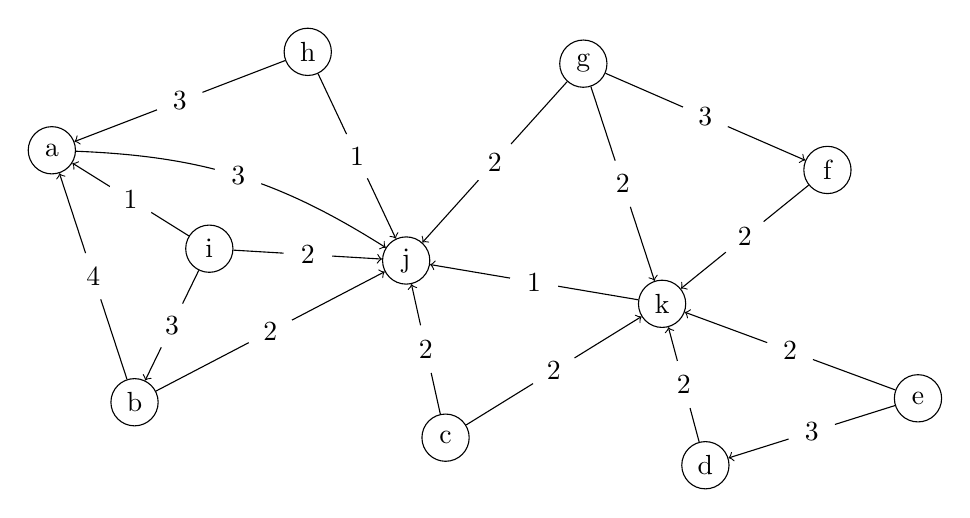
\begin{tikzpicture}
        % Nodes
        \node[circle, draw, minimum size=0.6cm, inner sep=0pt] at (0.5* 0.0, 0.5* 8.5)  (a)    {a};
        \node[circle, draw, minimum size=0.6cm, inner sep=0pt] at (0.5* 2.1, 0.5* 2.1)  (b)    {b};
        \node[circle, draw, minimum size=0.6cm, inner sep=0pt] at (0.5* 10.0, 0.5* 1.2)  (c)    {c};
        \node[circle, draw, minimum size=0.6cm, inner sep=0pt] at (0.5* 16.6, 0.5* 0.5)  (d)    {d};
        \node[circle, draw, minimum size=0.6cm, inner sep=0pt] at (0.5* 22.0, 0.5* 2.2)  (e)    {e};
        \node[circle, draw, minimum size=0.6cm, inner sep=0pt] at (0.5* 19.7, 0.5* 8.0)  (f)    {f};
        \node[circle, draw, minimum size=0.6cm, inner sep=0pt] at (0.5* 13.5, 0.5* 10.7)  (g)    {g};
        \node[circle, draw, minimum size=0.6cm, inner sep=0pt] at (0.5* 6.5, 0.5* 11.0)  (h)    {h};
        \node[circle, draw, minimum size=0.6cm, inner sep=0pt] at (0.5* 4.0, 0.5* 6.0)  (i)    {i};
        \node[circle, draw, minimum size=0.6cm, inner sep=0pt] at (0.5* 9.0, 0.5* 5.7)  (j)    {j};
        \node[circle, draw, minimum size=0.6cm, inner sep=0pt] at (0.5* 15.5, 0.5* 4.6)  (k)    {k};


        \draw[->]  (a) edge[bend left=15] node[circle, fill=white] {3} (j);

        \draw[->]  (b) edge node[circle, fill=white] {4} (a);
        \draw[->]  (b) edge node[circle, fill=white] {2} (j);

        \draw[->]  (c) edge node[circle, fill=white] {2} (j);
        \draw[->]  (c) edge node[circle, fill=white] {2} (k);

        \draw[->]  (d) edge node[circle, fill=white] {2} (k);

        \draw[->]  (e) edge node[circle, fill=white] {3} (d);
        \draw[->]  (e) edge node[circle, fill=white] {2} (k);

        \draw[->]  (f) edge node[circle, fill=white] {2} (k);

        \draw[->]  (g) edge node[circle, fill=white] {3} (f);
        \draw[->]  (g) edge node[circle, fill=white] {2} (j);
        \draw[->]  (g) edge node[circle, fill=white] {2} (k);

        \draw[->]  (h) edge node[circle, fill=white] {3} (a);
        \draw[->]  (h) edge node[circle, fill=white] {1} (j);

        \draw[->]  (i) edge node[circle, fill=white] {1} (a);
        \draw[->]  (i) edge node[circle, fill=white] {3} (b);
        \draw[->]  (i) edge node[circle, fill=white] {2} (j);


        \draw[->]  (k) edge node[circle, fill=white] {1} (j);
    \end{tikzpicture}
    \caption{Upward Graph des Beispielgraphs}
    \label{ch::fig::upward_graph}
\end{figure}

Die kürzeste Pfad Suche ist eine bidirectionale Suche, wobei die Suchen auf verschiedenen Graphen arbeiten.
Daher ist muss noch das Gegenstück das upward Graphens definiert werden, der \emph{downard Graph}.

\begin{definition}[Downward Graph]
    Sei $G = (V, E)$ und ${vtl} \coloneq V \to \mathbb{N}$ eine \emph{vertex-to-level} Funktion. Dann ist ein upward Graph des Umkehrgraphens $G^T$ ein \emph{downward Graph} zu $G$.
\end{definition}

Wenn ein Graph ungerichtet ist, dann er äuivalent zu seinem Umkehrgraphen.
Daher ist in so einem Fall dann auch der upward und downard Graph äuivalent.
Daher entspricht \autoref{ch::fig::upward_graph} gleichzeitig auch dem downward Graph des Beispielgraphens.

\section{Query}

Ein \emph{Contracted Graph} $C = (G_u, G_d)$ ist die Datenstruktur, mit deren Hilfe schnell kürzeste Wege gefunden werden können.
Sie besteht aus einem upwarward und downward Graph, wobei beide es eine ${vtl}$ Funktion geben muss, nach der Beide gültig sind.

Die Suche eines kürzesten Pfades von $a$ nach $e$ auf dem Beispielgraph gestaltet sich nun wie folgt:
Auf $G_u$ wird eine Breitensuche von $a$ und auf $G_d$ eine Breitensuche von $e$ durchgeführt.
Aus den von beiden besuchten Knoten wird derjenige ausgewählt, der die nidrigste Summe beider Distanzen hat.
Dieser Knoten auch auch das höchste Level auf dem Pfad.
\autoref{fig:ch:beispiel_suche} zeigt das auf- und absteigen der Level auf dem kürzesten Pfad.

\begin{figure}[ht]
    \centering
    \begin{tikzpicture}
        \node[circle, draw] at (0 * 1.5, -2 * 0.75)  (a)    {a};
        \node[circle, draw] at (1 * 1.5, -4 * 0.75)  (i)    {i};
        \node[circle, draw] at (2 * 1.5, -0 * 0.75)  (j)    {j};
        \node[circle, draw] at (3 * 1.5, -1 * 0.75)  (k)    {k};
        \node[circle, draw] at (4 * 1.5, -3 * 0.75)  (e)    {e};

        % draw axis
        \draw[->] (-1, -7 * 0.75) -- (-1, 0) node[above] {Level};

        \draw[->]  (a) -- (j);
        \draw[->]  (e) -- (k);
        \draw[->]  (k) -- (j);

        \draw[->, dotted]  (a) -- (i);
        \draw[->, dotted]  (i) -- (j);

    \end{tikzpicture}
    \caption{Beispiel einer Suche im Contrated Graph}
    \label{fig:ch:beispiel_suche}
\end{figure}

Diese informalle Beschreibung lässt sich formal definieren:

\begin{algorithm}
    \caption{Construction Hierachies Query}
    \begin{algorithmic}[1]
        \Require Upward-Graph $G_u = (V, E_u)$, Downward-Graph $G_d = (V, E_d)$, Startknoten $s \in V$, Zielknoten $t \in V$
        \Ensure Treffknoten $m \in V \cup \{ {none} \}$, ${dist}_u$, ${pre}_u$, ${dist}_d$, ${pre}_d$
        \State ${dist}_u$, ${pre}_u$ $\leftarrow$ Dijkstra$(G_u, s)$
        \State ${dist}_d$, ${pre}_d$ $\leftarrow$ Dijkstra$(G_d, t)$

        \State
        \State $m \leftarrow {none}$
        \State $d \leftarrow \infty$
        \State

        \ForAll {$v \in V$}
        \If {${dist}_u(v) + {dist}_d(v) < d$}
        \State $m \leftarrow v$
        \State $d \leftarrow {dist}_u(v) + {dist}_d(v)$
        \EndIf
        \EndFor

        \State
        \State \Return $m$, ${dist}_u$, ${pre}_u$, ${dist}_d$, ${pre}_d$
    \end{algorithmic}
    \label{ch:query_simple}
\end{algorithm}

Doch warum ist dies Korrekt?

\begin{beweis}
    Der Beweis der Korrektheit folgt in zwei Schritte.

    \begin{enumerate}
        \item
              Es existiert ein kürzester Pfad von $u$ nach $v$ in $G$ $\Rightarrow$ Er wird in $C$ gefunden.

              Da ${vtl}$ injektiv ist, existiert genau ein Knoten $t$ mit dem höchstem Level. Zerscheide den Pfad $(u, \dotsc, v)$ in zwei Teile:  und $(u, \dotsc, t)$ und $(t, \dotsc, v)$.

              Die Tupel benachbarten Knoten in $(u, \dotsc, t)$ sind nach der Definition des upward Graph Kanten von $G_u$. Daher wird $t$ im upward Graph gefunden.

              Analog dazu wird $t$ in $G_d$ gefunden, die Tupel benachbarter Knoten im Pfad $(v, \dotsc, t)$ sind nach der Definition des downward Graphs Kanten von $G_d$.

              Da die Tupel Kanten der Graphen sind, finden die Breitensuchen den Knoten $t$ mit minimalen Kosten ausgehend von $u$ bzw. $v$. Da $t$ auf dem kürzesten Pfad liegt, ist damit auch der kúrzeste Pfad von $u$ nach $v$

        \item
              Es existiert kein kürzester Pfad von $u$ nach $v$ in $G$ $\Rightarrow$ Es wird in $C$ kein Pfad gefunden gefunden.

              Angenommen, es würde ein Pfad in C gefunden werden. Die Tupel benachbarter Knoten des Pfades müssten dann Kanten in C sein.
              Mindestens einer diese Kanten hätte dann ein Gewicht welches gegen \autoref{ch:definition:legal_edges} der Definition verstoßt.
    \end{enumerate}

    Daher gilt, die Suche der kürzesten Pfad Distanz in $C$ ist äquivalent zu der in $G$
\end{beweis}

\subsection{Pfad gewinnung}
Bisher enthält der Pfad Shortcuts.
Entweder man ersetzt dan Shortcut auf einmal durch alle Knoten, oder iterativ durch jeweils zwei Kanten.

Diese müssen ersetzt werden.
Das geht, indem einen Stapel hat und shortcuts einfügt.

\section{Early stop}

Dass beide Suchen vollständig asugeführt werden ist nicht optimal.
Besser wäre es, frühzeitig stoppen zu können.
Vielleicht, wenn ein Knoten $t$ mit Distanz $d$ gefunden wurde.
Dann stoppen wenn top queue forward + top queue reverse >= d?
Das funktioniert nicht.
Denn bei der während bei einer normalen bidirectionale Suche sich die Fronten treffen, kann eine CH suche auch hinter die Front der anderen gelangen.

Daher ist die Abbruchbedingung: top queue >= d.

Todo: Abbruch mit Heuristik. Wenn ich upper bound kenne. breche ab top queue >= upper bound.

\todo{Funke fragen}.

\section{Pruning}


% https://cstheory.stackexchange.com/questions/23767/why-is-label-pruning-possible-with-hub-labeling
Aus dieser Definition folgt, dass der kürzeste Pfad zwischen zwei Knoten in $G_u$ ist also mindestens genausolang ist wie in $G$.
Der Pfad darf aber auch länger sein.

\todo{Zeiche zwei Suchbäume, jeweils in G und Gu}

Für die Suche sind aber nur Knoten interesannt, die tatsächlich kürzesten Pfad Abstand haben.

Wie kann man diese Knoten nun leicht rausfiltern?
Beim expanded eines Knoten prüft man, für die Nachbarn der Gegenrichtung:
\todo{Funke nochmal die Details}


\section{Erstellung}

Das Ziel der Contraction Hierarchies ist es aus dem Graph zwei Teilgraphe mit Abkürzungen (\emph{shortcuts}) zu erstellen.
Auf diesen Graphen kann mit einer Breitensuche effizient ein Knoten gefunden werden, der auf dem kürzesten Pfad zwischen zwei Knoten liegt.

\subsection{Contraction}

Der Name Contraction Hierachies leitet sich aus Konzept der Knoten Kontraktion (contraction) ab.
Diese funktioniert wie folgt:

\begin{definition}[Vertex Contraction]
    Sei $G = (V, E)$ ein Graph. Sei $v \in V$ der zu kontraktierende Knoten. Er wird kontraktiert indem:

    \begin{enumerate}
        \item\label{ch:contraction:when_shortcut}
        für jeden Vorgänger $u \in V$ und jeden Nachfolger $w \in V$ von $v$ einen Kante $(v, w, {spd}(u, w))$ in $E$ eingefügt wird, wenn $v$ auf dem einzigen kürzesten Pfad zwischen $u$ und $v$ liegt. Diese Kanten sind Shortcuts.

        \item
              alle Kanen von und zu $v$ entfernt werden.
    \end{enumerate}

    $v$ ist danach isoliert.
\end{definition}

Diese Operation erhält für die verbleibenden Knoten die kürzesten Pfade.
Betrachten wir dies wieder am Beispielgraph.
Sei $i$ der zu kontraktierende Knoten, die Nachbarn sind $a$, $b$, $j$ und $h$.
Die kürzesten Pfade von $(a, b)$, $(b, j)$, $(h, j)$ und $(a, h)$ fürhren nicht durch $i$.
Der von $(a, j)$ jedoch doch, daher wird eine Kante eingefügt.
\autoref{graphs:fig:example_contraction} zeigt den Graphen nach der Kontraktion.

\begin{figure}[ht]
    \centering
    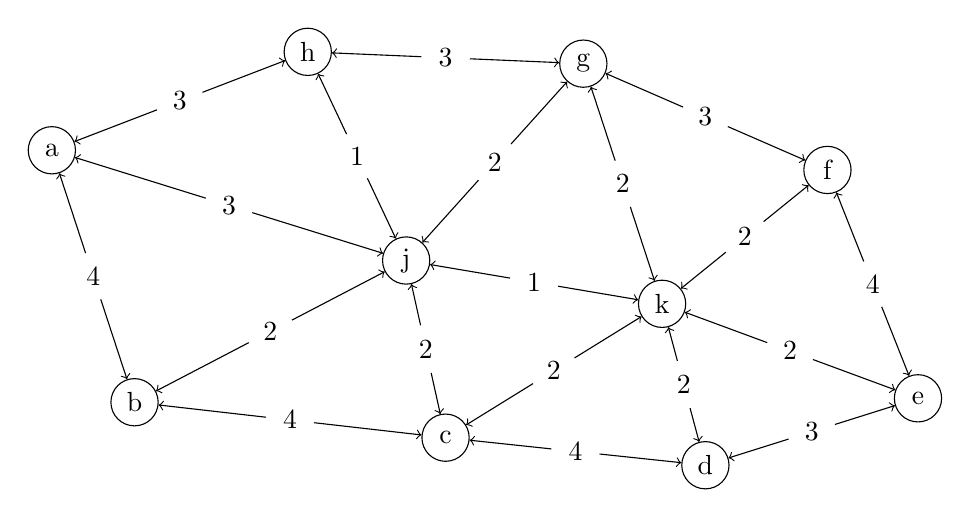
\begin{tikzpicture}
        % Nodes
        \node[circle, draw, minimum size=0.6cm, inner sep=0pt] at (0.5* 0.0, 0.5* 8.5)  (a)    {a};
        \node[circle, draw, minimum size=0.6cm, inner sep=0pt] at (0.5* 2.1, 0.5* 2.1)  (b)    {b};
        \node[circle, draw, minimum size=0.6cm, inner sep=0pt] at (0.5* 10.0, 0.5* 1.2)  (c)    {c};
        \node[circle, draw, minimum size=0.6cm, inner sep=0pt] at (0.5* 16.6, 0.5* 0.5)  (d)    {d};
        \node[circle, draw, minimum size=0.6cm, inner sep=0pt] at (0.5* 22.0, 0.5* 2.2)  (e)    {e};
        \node[circle, draw, minimum size=0.6cm, inner sep=0pt] at (0.5* 19.7, 0.5* 8.0)  (f)    {f};
        \node[circle, draw, minimum size=0.6cm, inner sep=0pt] at (0.5* 13.5, 0.5* 10.7)  (g)    {g};
        \node[circle, draw, minimum size=0.6cm, inner sep=0pt] at (0.5* 6.5, 0.5* 11.0)  (h)    {h};
        % \node[circle, draw, minimum size=0.6cm, inner sep=0pt] at (0.5* 4.0, 0.5* 6.0)  (i)    {i};
        \node[circle, draw, minimum size=0.6cm, inner sep=0pt] at (0.5* 9.0, 0.5* 5.7)  (j)    {j};
        \node[circle, draw, minimum size=0.6cm, inner sep=0pt] at (0.5* 15.5, 0.5* 4.6)  (k)    {k};


        \draw[<->]  (a) edge node[circle, fill=white] {4} (b);
        \draw[<->]  (a) edge node[circle, fill=white] {3} (h);
        \draw[<->]  (a) edge node[circle, fill=white] {3} (j);

        \draw[<->]  (b) edge node[circle, fill=white] {4} (c);
        \draw[<->]  (b) edge node[circle, fill=white] {2} (j);

        \draw[<->]  (c) edge node[circle, fill=white] {4} (d);
        \draw[<->]  (c) edge node[circle, fill=white] {2} (j);
        \draw[<->]  (c) edge node[circle, fill=white] {2} (k);

        \draw[<->]  (d) edge node[circle, fill=white] {3} (e);
        \draw[<->]  (d) edge node[circle, fill=white] {2} (k);

        \draw[<->]  (e) edge node[circle, fill=white] {4} (f);
        \draw[<->]  (e) edge node[circle, fill=white] {2} (k);

        \draw[<->]  (f) edge node[circle, fill=white] {3} (g);
        \draw[<->]  (f) edge node[circle, fill=white] {2} (k);

        \draw[<->]  (g) edge node[circle, fill=white] {3} (h);
        \draw[<->]  (g) edge node[circle, fill=white] {2} (j);
        \draw[<->]  (g) edge node[circle, fill=white] {2} (k);

        \draw[<->]  (h) edge node[circle, fill=white] {1} (j);

        \draw[<->]  (j) edge node[circle, fill=white] {1} (k);
    \end{tikzpicture}
    \caption{Beispielgraph}
    \label{graphs:fig:example_contraction}
\end{figure}

Um einen Contracted Graph zu erstellen, werden alle Knoten kontraktiert, wobei die Kanten, die in jedem Schritt entfernt werden, gesammelt werden.
Die Kanten, deren Kopf-Level größer ist, bilden die Kanten des upward Graphens.
Die übrigen Kanten, also die deren Fußlevel größer ist, werden invertiert und bilden die Kanten des downard Graphens.

Diese Art der Erstellung erzugt zulässige upward Graphen, da die eingefügten Shortcuts die die Bedingung aus \autoref{ch:definition:upward} erfüllen.
Es ist jedoch möglich, dass Kanten eingefügt werden, die nicht notwendig sind.
Insbesondere hat die Reihenfolge der Kontraktion einen großen Einfluss auf die Qualität der erzeugten Graphen.
\todo{Wie definiere ich die Qualität}?

Die Suche in der Kontraktion wird häufig wie folgt gestalltet.
Es wird eine one-to-many Suche gemacht, welche auf zwei Arten limitiert ist:
Es wird nur der Ball mit Abstand der gößten Distanz out-Kanten + in-Kante abgesucht.
Die Anzahl der Hops wird begrenzt.
Dadurch werden im Zweifelsfall mehr Kanten als benötigt eingefügt, dies ist aber schneller.

\subsubsection{Top-Down}

Bei der Top-Down Contraction ist level-to-vertex Funktion ${ltv}$ vorgegeben.
Die Knoten werden in Reihenfolge ihres Levels kontrakiert, wobei mit dem niedrigsten Level begonnen wird.

\paragraph{Zufällig sortiert}
Die Knoten werden zufällig auf die Level verteilt

\paragraph{Sortiert nach Grad}
Die Knoten werden nach ihrem Grad sortiert, wobei die kleinsten Grade zuerst kontraktiert werden.
Die überlegung dahinter ist, dass Knoten mit vielen Nachbarn auch viele neue Kanten einfügen können, was vermieden werden soll.

\paragraph{Hitting Set}
Es wird ein Hitting Set über Pfade in $G$ erstellt.
Die Knoten welche am wenigsten Pfade treffen, werden zuerst kontraktiert.
Dies ist potentiell eine der besten Lösungen \todo{Oder? Kann man das beweisen?}.

\subsubsection{Bottom-Up}

Bei der Bottom-Up contraction wird die vertex-to-level Funktion ${vtl}$ währen der Kontraktion erstellt.
Dafür wird mit einer Heuristik der jeweils nächst \emph{unwichtigste} Knoten ausgewählt, kontraktiert und dem nächstem Level zugewiesen.
Ein unwichtiger Knoten hat hierbei einen niedrigen Heuristik-Wert.
Hier hängt die Qualität der des Ergebnis von der Heuristik ab.

Da das Neuberechnen des Heuristik für alle Knoten im Allgemeinen zu teuer ist, werden zwei Methoden angewendent:
Beim \emph{Lazy poping} besteht die Annahme, dass ein Knoten nur wichtiger werden kann.
Aus der Warteschlange wird ein Knoten entnommen und geprüft, ob sein Heuristik-Wert noch gleich ist.
Wenn er noch gleich ist, wird er kontraktiert, wenn nicht wird er zurück die Warteschlange gepusht.
Dies wird wiederholt, bis schließlich ein Knoten gefunden wird.
Beim \emph{Neighbor update} werden nach der Kontraktion eines Knoten die Heuristik Werte der Nachbarn geupdated.

Es sind viele Heurisiken Möglich, die auch kombiniert werden können.
Die in der Praxis am meist-verwendet Heurisik ist die \emph{Kanten-Differenz}.
Sie gibt an wie sich die Anzal der Kanten im gesammten GRaph verändert
Sie wird durch die Anzahl der hinzugefügten Kanten subtrahiert durch die Anzalh der entfernten Kanten gebildet.
Hierfür wird die Kontraktion eines Knoten simuliert.

\subsubsection{Ideen}

Die bisher erwähnten Methoden eignen sich nur bedingt für graphen mit großem durchscnittlichen Knotengrad.
Für die Kontraktion muss jeweils für jeden Vorgänger eine Suche zu jedem Nachfolger gemacht werden.
Insbesonder für Sichtbarkeitsgraphen ist das sehr teuer.

Es gibt zwei Stellen, die beschleunigt werden müssen:
Ordering Heuristik und Kontraktion

\paragraph{Kontraktion}
Anstatt einer Suche, verwende eine Upper Bound Heuristic.
Es muss ein Shortcut eingefügt werden, wenn die Shortcut Distanz gleich der Wahren Distanz ist.
Dies ist erfüllt, wenn die Shortcut Distanz kleiner gleich einer Upper Bound ist.
Zusätzlich gilt, wenn lower bound == shortcut distanz, dann muss Shortcut eingefügt werden.

Dafür gibt es zwei Ideen, die kombiniert werden können.
Landmarks und eine CH/HL des triangulierten Graphes für den Sichtbarkeitsgraph.
Vielleicht gilt, dass Landmarks für größere Entfernungen / mehr Hops gut ist und CH/HL für kleine?

Alternativ, aber wahrscheinlich super doof:
Füge jeden Shortcut ein.

Heuristic.
Statt suche kann man auch heursitc benutzten.

Used heuristics:
TrivialeHeuristic (all in). Füge jeden shortcut ein.

\paragraph{Ordering Heuristik}
Wähle $n$ Paara aus Vorgänger Nachgänger aus und erstelle für diese Edge Differnce (wieder mit Heuristik).
\todo{plot genauigkeit vs Zeit, vielleicht über so 1000 Knoten?}

\section{Brute force}

Die upward Graphen können auch stumpf berechnet werden.
Dafür wird pro Knoten eine (zwei, upward, downard) Dijsktrasuche gemacht, bis alle Knoten nach der Bedingung gefunden werden.


Dafür wird während der Dijstra Suche notiert, was das größte Level auf dem Weg von der Wurzel bis zu dem Knoten ist.
Ein Knoten ist der Kopf eine CH Kante, für die gilt, dass das größte Level auf dem Weg zur Wurzel zu ihr sie selber hat und der größte Level des Vorgängers der der Wurzel ist.
Das Gewicht der Kante kann Dijkstra entommen werden.
Wenn für Knoten ein max Level auf dem Pfad haben, welches größer als das der Wurzel ist, kann abgebrochen werden.

Die Shortcuts können dabei auch erstellt werden.
Der zu shortcutende Knoten ist der, mit demm dritthöchstem Level dazwischen.
Die anderen müssen auch erstellt werden, denn sonst kannes Probleme geben: \todo{Bild}

Das mit den Shortcuts ist dann nicht so einfach. TODO Bild

